The refrigeration trailer (hereinafter referred to as reefer trailer) is an insulated trailer designed and built by Schmidt Cargobull with a cooling system developed by Bitzer. It is attached to a truck and has a length of 13.4 meters. The trailer features room for 33 Euro-pallets of cargo and is used to transport various goods that require specific  conditions during transportation, e.g. temperature, humidity and CO2 level. The cooling system used to control the internal temperature in the trailer is powered by an internal battery. This allows the reefer trailer cooling to be powered independently of the truck.

While a reefer trailer usually has its own cooling system installed, the reefer trailer in this project utilizes a custom HVAC system designed by BITZER. This system is built to facilitate testing of advanced control strategies.

\subsection{Refrigeration Systems}
The role of a refrigeration system resides in the second law of thermodynamics. It can be formulated in many ways, one of which is that heat transfer always happens from a warmer to a colder body but never in the reverse direction. This essentially motivates a refrigeration system as the objective is extract heat from a cold to a warm body, e.g. from cargo in a reefer trailer to the surrounding ambient air.

\subsubsection{Principle of refrigeration}
A textbook example of a refrigeration system is a single stage refrigeration system as depicted in \cref{fig:HVAC_Diagram_std}. It is comprised of 4 components, a compressor, an expansion valve, and two heat exchangers, the evaporator and the condenser. Assuming that the pressure loss in evaporator and condenser is negligible, there will be a high pressure side and a low pressure side of the refrigeration circuit. The high pressure side accommodates that the refrigerant temperature is increased above the hot body temperature, thus allowing for heat transfer from refrigerant to hot body. On the low pressure side, the refrigerant temperature is less than the cold body, which enables heat transfer from cold body to the refrigerant. In order to further describe the refrigeration process, a pressure-enthalpy diagram (p-h diagram) is consulted.
\begin{figure}[h]
	\centering
	\begin{minipage}{0.5\textwidth}
		\centering
		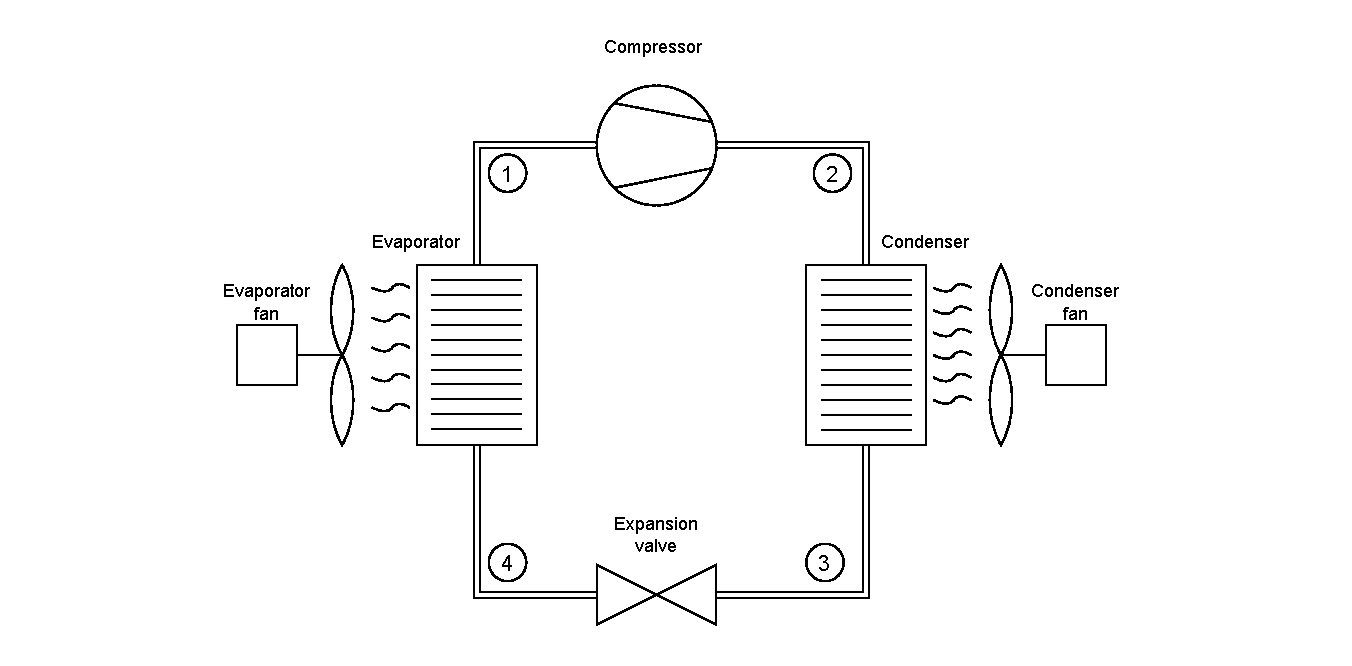
\includegraphics[width=1\textwidth]{Graphics/HVAC_Diagram_std.pdf} % first figure itself
		\caption{Illustration of single stage refrigeration cycle}
		\label{fig:HVAC_Diagram_std}
	\end{minipage}\hfill
	\begin{minipage}{0.5\textwidth}
		\centering
		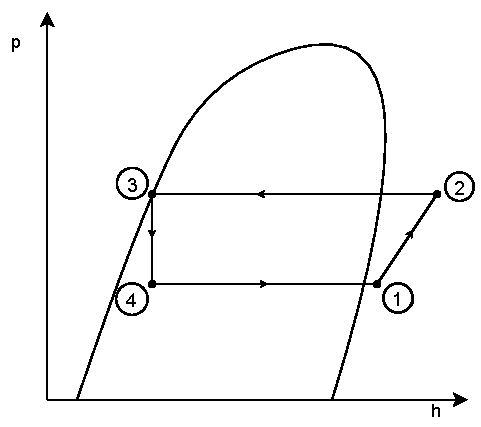
\includegraphics[width=1\textwidth]{Graphics/p-h_diagram_std} % second figure itself
		\caption{Illustration of p-h diagram of single stage refrigeration cycle}
		\label{fig:p-h_diagram_std}
	\end{minipage}
\end{figure}
The pressure and enthalpy of the refridgerant as it moves around in the refrigeration cycle are illustrated in \cref{fig:p-h_diagram_std}. The four connection points between the components in \cref{fig:HVAC_Diagram_std} are illustrated. 

\begin{itemize}
	\item From point 1 to 2 the compressor increases the pressure (and enthalpy) of the vapor refrigerant. The increase in enthalpy is not desired, but cannot be omitted as it is not an isenthalpic process. The compressor also drives the flow of refrigerant in the circuit.
	\item From point 2 to 3 the high pressure and high temperature vapor refrigerant runs through the condenser and heat is transferred to the ambient. This is an isobaric exothermic process. The refrigerant is intended to change phase from vapor to liquid, hence the name condenser.
	\item From point 3 to 4, the high pressure but low enthalpy liquid refrigerant passes through an isenthalpic expansion, which lowers the pressure and thereby also the temperature. Some of the liquid may change phase to gas, s.t. the refrigerant is now a mix of vapor and liquid.
	\item From point 1 to 4, the low pressure and low temperature liquid-vapor refrigerant runs through the evaporator and heat is transferred from the load to the refrigerant. The refrigerant completely changes phase to vapor. This is an isobaric endothermic process. 
\end{itemize}
 
\subsubsection{The BITZER Refrigeration System}
The refrigeration system implemented in the trailer used in this project contains more components than the standard example. An seen in \cref{fig:HVAC_Diagram}, the compressor is comprised of two stages, rather than one. Similarly two valves are being used. The valves are separated by a flash tank, that enables flash gas from the condenser throttle valve to the second stage of the compressor. The removed flash gas ensures that the liquid refrigerant that enters the evaporator has lower enthalpy and thereby higher cooling capacity. This enables higher efficiency of the system than a single stage system.\\
The subcooling throttle valve is only used for debugging purposes, and is fully open at all times in this project. The reefer system has two fans that enables variable amounts of forced convection instead of natural convection. The heat transfer coefficients from the heat exchangers (evaporator and condenser) to the cold and hot body can such be varied with the fan speed.

\begin{figure}[h]
	\centering
	\begin{minipage}{0.6\textwidth}
		\centering
		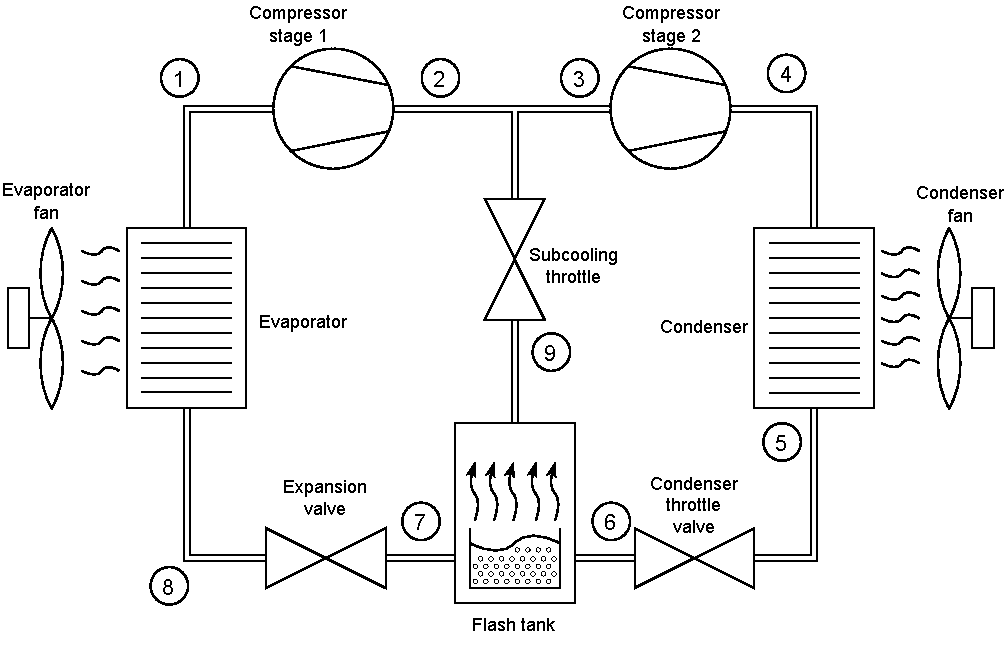
\includegraphics[width=1\textwidth]{Graphics/HVAC_Diagram_Fans.pdf} % first figure itself
		\caption{Illustration of two stage refrigeration circuit}
		\label{fig:HVAC_Diagram}
	\end{minipage}\hfill
	\begin{minipage}{0.4\textwidth}
		\centering
		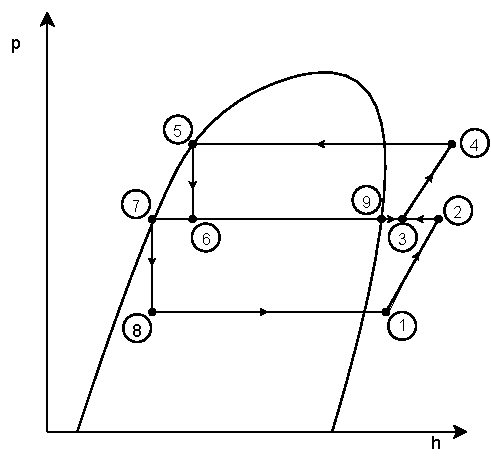
\includegraphics[width=1.05\textwidth]{Graphics/Flash_Tank_P-h_Diagram} % second figure itself
		\caption{Illustration of p-h diagram of two stage refrigeration circuit}
		\label{fig:p-h_diagram}
	\end{minipage}
\end{figure}

In \cref{fig:p-h_diagram} an illustrative p-h diagram of this refrigeration cicuit can be seen. The numbers in the figure are also shown in \cref{fig:HVAC_Diagram} for reference. Two loops can be observed on the diagram. The first is the outer loop from point $1 \rightarrow 2\rightarrow 3 \rightarrow 4 \rightarrow 5 \rightarrow 6 \rightarrow 7 \rightarrow 8 \rightarrow 1$. This is considered the primary loop. The second loop is the inner loop running from $3 \rightarrow 4 \rightarrow 5 \rightarrow 6 \rightarrow 9 \rightarrow 3$. \\
The refrigeration system essentially works as a single stage system, however the compression and expansion is distributed along two stages.

\begin{itemize}
	\item From point 1 to 2, the low pressure high enthalpy vapor refrigerant from the evaporator is compressed. The output vapor refrigerant is at medium pressure and medium enthalpy. 
	\item From point 2 and 9 to 3, the compressor stage 1 output refrigerant is mixed with the flash gas from the flash tank. 
	\item From point 3 to 4, the medium pressure and enthalpy vapor refrigerant mix is compressed further, outputting high pressure and enthalpy vapor refrigerant.
	\item From point 4 to 5, the high pressure and enthalpy vapor refrigerant is condensed through the condenser, which decreases the enthalpy. This is where the heat from the load is transferred to the ambient air (hot body).
	\item From point 5 to 6, the pressure decreased of the high pressure low enthalpy liquid refrigerant. This results in a medium pressure low enthalpy refrigerant where some of the refrigerant has changed phase to vapor.
	\item From point 6 to 7 and 9 \todo[inline]{Write about the last couple of stages}
\end{itemize}

The system components have variables that can be set to control their behavior. These are the controlled inputs:

\begin{itemize}
	\item The compressor speed $ \omega $
	\item The condenser fan speed $ U_{fan1} $
	\item The evaporator fan speed  $ U_{fan2} $
	\item The condenser throttling valve opening degree $ \Theta_1 $
	\item The expansion valve opening degree $ \Theta_2 $
\end{itemize}

There are several variables such as pressure and temperature throughout the refrigeration cycle, which are measured and hence are outputs of the system. \todo[inline]{mention which}

The controlled outputs however, are those of interest from a control point of view. These are the outputs that the control strategy seeks to keep at a set point. In this project it will be the trailer box air temperature and the evaporator superheat. Controlling the air temperatur is nessesary to ensure proper storage conditions for the cargo. Regulating the superheat is a more complex objective, as having a large amount of superheat is wasteful and decreases the overall energy efficiency of the trailer. There should however be some amount of superheat, to ensure no liquid refridgerant enters the compressor, since that is destructive to the mechanical system.\\

The aim of the project is to design a Multiple-Inputs-Multiple-Outputs (MIMO) state space controller to keep the temperature inside the container constant despite exogenous inputs (disturbances), specifically the ambient temperature. Furthermore it should do so with the sub-goal of minimizing the energy consumption, primarily by regulating the superheat.\\





\subsection{High-Fidelity model}
When working with a any large scale plant, testing iteratively on the physical system is often impractical. Slow dynamics and inconvienient test procedures make the proces tedious for the user, but there is also the risk of equipment damage. Therefore, it is common practice to develop a high-fidelity model of the system. Testing can be performed efficiently and with no risk on the model. \\

BITZER has created such a Hi-Fi model for the cooling trailer in Simulink. The model has been shown to be highly accurate and can be trusted to mimic the real system behavior in most use-cases. The Hi-Fi model simulates the refridgeration system in \cref{fig:HVAC_Diagram}. The controlled inputs are regulated by a decoupled PID network. The cargo hold air temperature is regulated to -5$^{\circ}$C.\\

The control strategy developed in this project, will first and foremost be tested on the Hi-Fi model. 




\subsection{Problem structure}

The controller will require access to relevant system information. In the context of state space control, this is the values of the system states. The states will be discussed in details later in the report. The states are used for feedback when choosing the proper control signals. Since the states of complex systems are usually not directly measurable, a simple model will be developed for state observation. The model is then to be used for controller design. \\

The control model will be developed by means of first principle modelling. Doing so yields a non-linear model, due to the non-linear physical properties of thermodynamical systems. To apply linear control strategies, the model must be linearised. Optimal control strategies will be implemented on the linear model, as the control objectives can be well formulated as an optimization problem. The optimization problem in this project will be to keep the controlled outputs fixed, while minimizing the energy consumption of the system.\\


		
